%!TEX root = ../../../memoria.tex
\section{\checkoutEF}\label{chapter:solucionimplementada:section:checkout}

	Una de las peores violaciones de usabilidad para un \websiteINT \ecommerceCOM corresponde a un proceso de \checkoutEF que no sea lineal. \websiteINT que no tengan un proceso de \checkoutEF lineal deja a muchos de los usuarios confusos e intimidados. Al momento de realizar este estudio, tanto \walmartNAME como \zapposNAME tenían un proceso \checkoutEF no lineal \cite{online_official_smashingmagazine_fundamental_guidelines_checkout_design}.
	% One of the worst usability violations that we discovered in our testing was non-linear checkout processes. Websites with a non-linear checkout process left several of our test subjects confused and intimidated. At the time of testing, both Walmart and Zappos had a non-linear checkout process.

	% The typical way to “accidentally” end up with a non-linear checkout process is to create steps within steps. This happens, for example, when the customer has to set a “Preferred shipping address” (Walmart’s violation) or “Create an account” (Zappos’ violation) on a separate page, and is then redirected to a previous checkout step upon completion.
	% Below, you can see Walmart’s checkout flow in thumbnails (click image for larger view). Notice that it’s non-linear because the “Preferred shipping address” sub-step directs the user to a previous step:

	Afortunadamente, hacer el proceso completamente lineal no es difícil. En el caso de necesitar, por ejemplo, un \subPasoCPT tal como \textit{creación de una cuenta}, esta nunca debe redirigir a un paso previo en el proceso de \checkoutEF, en lugar de eso, debe dirigir al cliente al siguiente paso del proceso \cite{online_official_smashingmagazine_fundamental_guidelines_checkout_design}. 
	%Luckily, making the process completely linear is easy. In this case, a sub-step such as “Account creation” should never redirect to a previous step in the checkout process, but instead direct the customer to the next step in the checkout process.

	Esto es crítico porque el modelo mental de la mayoría de los compradores dicta que el proceso de \checkoutEF debería ser lineal. Al ver la misma página dos veces, la mayoria de los clientes concluye que el sitio tiene un error, porque esto ocurre cuando hay errores de validación. \cite{online_official_smashingmagazine_fundamental_guidelines_checkout_design}. 
	%This is critical because the mental model of most customers dictates that a checkout process should be linear. Upon seeing the same page twice, most customers would conclude that the website has an error, because this is what happens with validation errors.
	%As one test subject said, “This looks suspiciously like the page I was on before. Is there something I didn’t do correctly?”

	Para este \frameworkPC se ha implementado un proceso de \checkoutEF lineal, el cual tiene los pasos que se aprecian en la \refFigura{figure:checkout:steps}.

	% \begin{figure}[H]
	% 	\centering
	% 	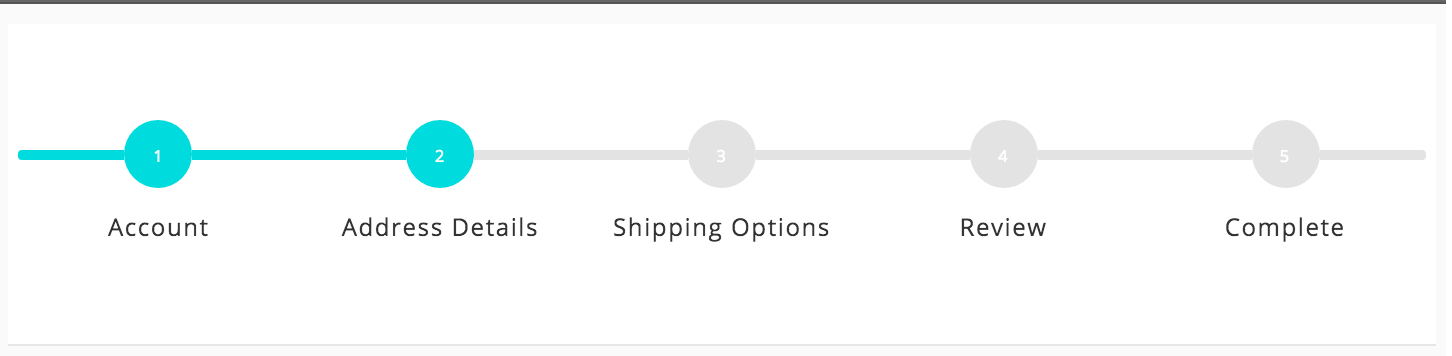
\includegraphics[width=0.7\textwidth]{figuras/shipping/global_status.png}
	% 	\caption{Estado actual del \workflowCPT del \shippingEF. En este caso se encuentra en la selección de la dirección.}
	% 	\label{figure:checkout:global_status}
	% \end{figure}

	\begin{figure}[!h]
		\centering
		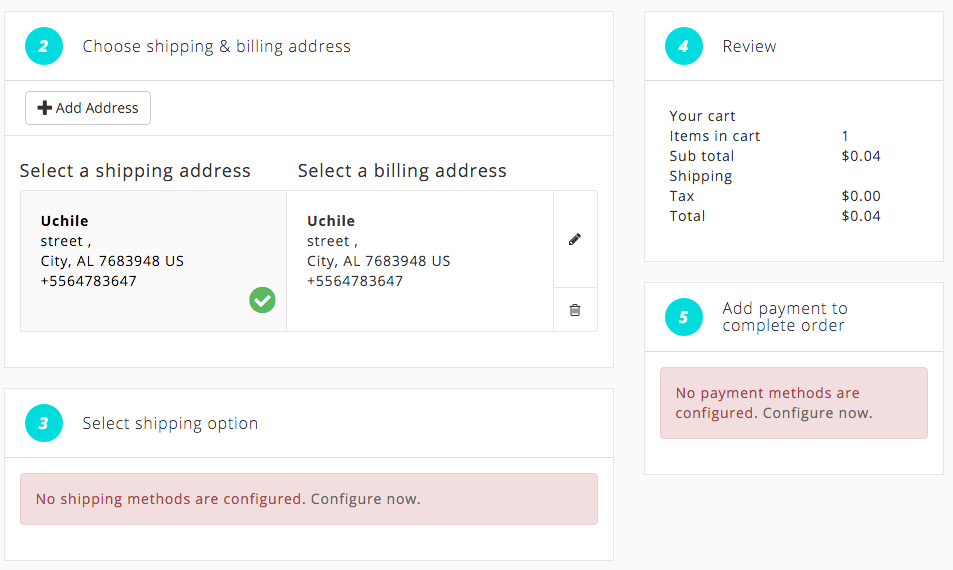
\includegraphics[width=0.8\textwidth]{figuras/shipping/steps.png}
		\caption{Detalle de todos los pasos del \workflowCPT \shippingEF.}
		\label{figure:checkout:steps}
	\end{figure}

	Otro detalle importante a considerar es que mientras sea posible hay que limitar el proceso de \checkoutEF a una sola página. En el caso de separar el proceso en algunas páginas, se debe incluir una barra de proceso para mostrar cuanto falta para terminar \cite{online_official_imediaconnection_best_practices_shopping_cart}.
	% Try to keep it to one page
	% If at all possible, limit the checkout process to a single page. If you must spread it out across a few pages, include a progress bar to show people how far they have left to go.
	% Read more at http://www.imediaconnection.com/content/36794.asp#6qlTEqOcCeTePmFQ.99

	Afortunadamente, ambas restricciones son una manera para lograr la otra. Por lo tanto se desarrollá el proceso incluyendo a ambas. Esto se observa en la \refFigura{figure:checkout:global_status}.

	\begin{figure}[H]
		\centering
		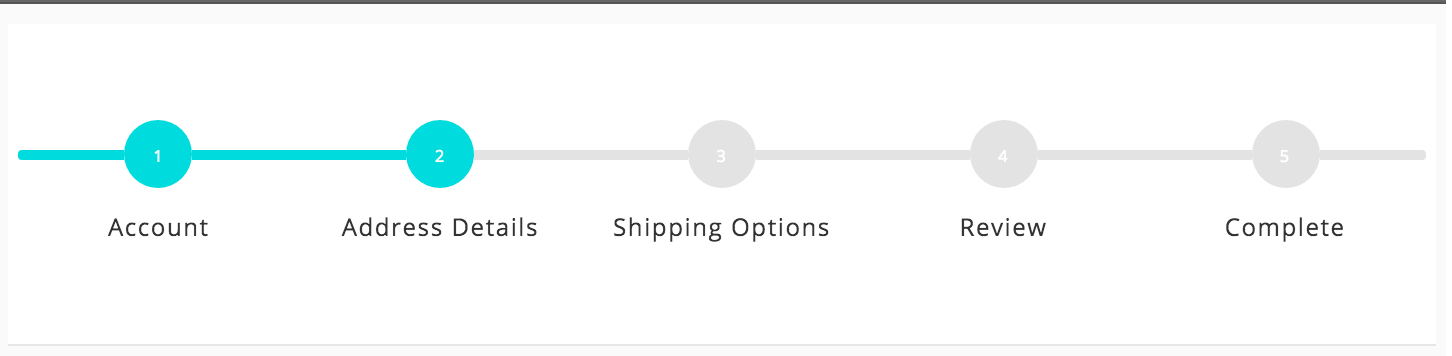
\includegraphics[width=0.7\textwidth]{figuras/shipping/global_status.png}
		\caption{Estado actual del \workflowCPT del \shippingEF. En este caso se encuentra en la selección de la dirección.}
		\label{figure:checkout:global_status}
	\end{figure}

	Cada uno de los pasos que aparecen en la \refFigura{figure:checkout:steps} son descritos a continuación.

	% Paso Cuenta de usuario
	%!TEX root = ../../../../memoria.tex
\subsection{Cuenta de usuario}\label{chapter:solucionimplementada:section:account}

	Nada irrita más a un cliente que ser forzado a crear una cuenta para lograr comprar algo \online. Despues de todo, comprar \online se supone debería ser sencillo. Es cierto que la creación de una cuenta hará que las comprar en el futuro sean mas sencillas, pero no aporta nada para la situación en cuestión \cite{online_official_imediaconnection_best_practices_shopping_cart}.
	% Don't require registration to complete checkout
	% Nothing irks a customer more than being forced to create an account in order to buy something online. After all, online shopping is supposed to be easy. Sure, having an account will make future purchases easier, but it does nothing for the situation at hand. Instead, give shoppers the option of creating an account once the transaction is complete.

	Es cierto que este \frameworkPC requiere la creación de una cuenta para lograr la compra de productos, sin embargo no es necesario confirmarla para poder comprar. Es cierto que esta no es la situación ideal, pero esta situación tampoco es del todo mala, dado la simplicidad en la \nameref{chapter:solucionimplementada:accounts:subsection:create} (\ref{chapter:solucionimplementada:accounts:subsection:create}). 

	% Paso selección shipping & billing address
	%!TEX root = ../../../../memoria.tex
\subsection{Detalles de dirección}\label{chapter:solucionimplementada:section:address}

	Esta sección funciona exactamente igual \nameref{chapter:solucionimplementada:section:profile:subsection:book_address} ( \ref{chapter:solucionimplementada:section:profile:subsection:book_address}). En otras palabras, aparte de seleccionar una direacción permite:

	\begin{itemize}
		\item Ver todas las direcciones configuradas en el sistema.
		\item Editar y/o eliminar las direcciones disponibles del sistema.
		\item Configurar una nueva dirección.
		\item En caso de no tener ninguna dirección configurada, muestra el fomulario de creación.
	\end{itemize}

	Como se indica en otras partes, es altamente deseable limitar el proceso de \checkoutCOM a una sola página \cite{online_official_imediaconnection_best_practices_shopping_cart}. Estas funcionalidades están alineadas con este principio. En caso de necesitar hacer alguna gestión en las direcciones, no sea necesario cambiar de página.
	Como ejemplo, en la \refFigura{figure:checkout:form_address_default} se observa el formluario de creación de una dirección dado que no existe ninguna configurada previamente.

	\begin{figure}[H]
		\centering
		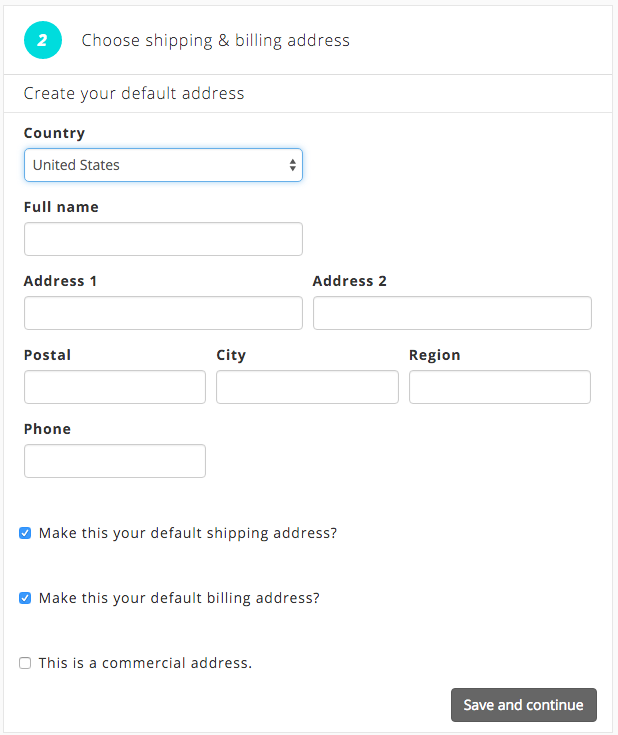
\includegraphics[width=0.6\textwidth]{figuras/shipping/form_address.png}
		\caption{Despliegue automático del formulario de direcciones cuando no se tienen ninguna dirección agregada.}
		\label{figure:checkout:form_address_default}
	\end{figure}

	% Paso opciones de envío
	%!TEX root = ../../../../memoria.tex
\section{Opciones de \ShippingCOM}\label{chapter:solucionimplementada:section:shipping_options}

	En este paso es posible seleccionar alguno de los métodos disponibles de \ShippingCOM por el sitio de ventas (\refFigura{figure:shipping:checkout:select_option}). Como describió en la sección 

	\begin{figure}[!h]
		\centering
		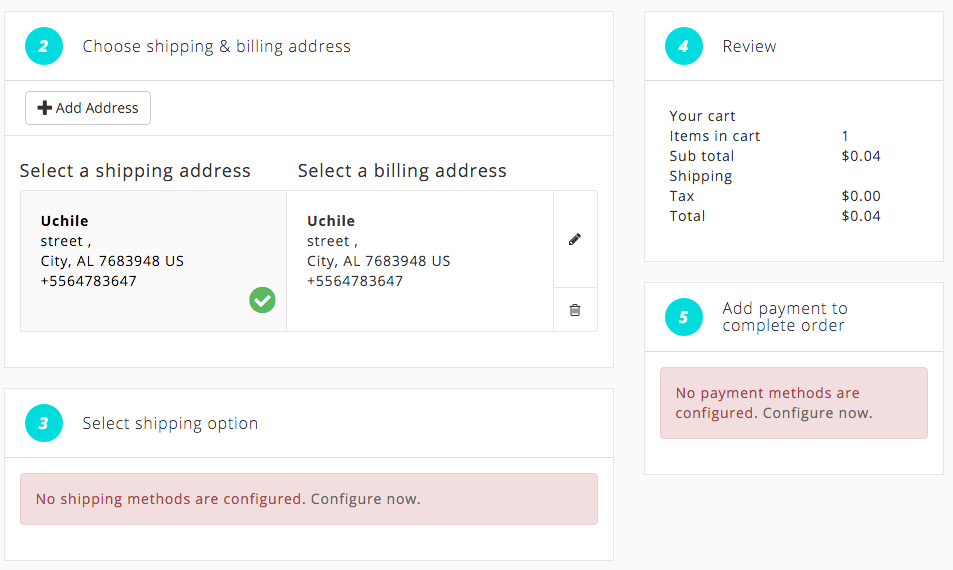
\includegraphics[width=0.8\textwidth]{figuras/shipping/steps.png}
		\caption{Detalle de todos los pasos del \workflowCPT \shippingEF.}
		\label{figure:shipping:checkout:select_option}
	\end{figure}

	% Paso resumen de la compra
	%!TEX root = ../../../../memoria.tex
\subsection{Resumen de la compra}\label{chapter:solucionimplementada:checkout:review}

	Esta sección muestra un resumen de la compra que se esta realizando (ver \refFigura{figure:review:checkout:summary}). Esta información es parte del detalle completo que debe mostrar esta sección para dejar claro al cliente que es exactamente lo que esta comprando. Esto debe ser mejorado como trabajo futuro.

	\begin{figure}[!h]
		\centering
		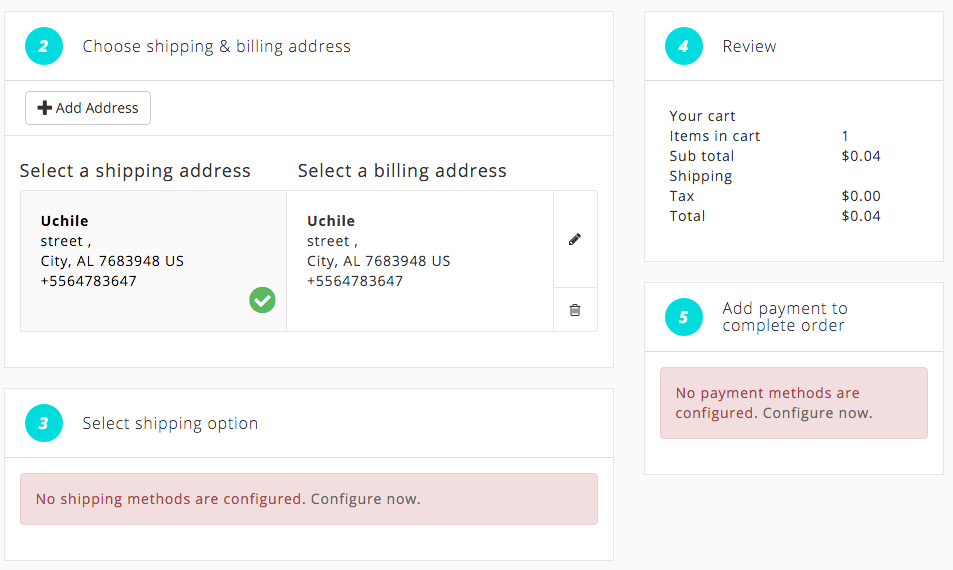
\includegraphics[width=0.8\textwidth]{figuras/shipping/steps.png}
		\caption{Detalle de la compra dentro del proceso de \checkoutEF.}
		\label{figure:review:checkout:summary}
	\end{figure}

	% Paso add paymant to complete order
	%!TEX root = ../../../../memoria.tex
\subsection{\paymentsCOM}\label{chapter:solucionimplementada:section:payment}
	
	Como se mencionó en la sección \ref{cap:solucionImplementada:section:dashboard:subsection:payment} \nameref{cap:solucionImplementada:section:dashboard:subsection:payment}, es relevante considerar varios métodos de pagos, sin embargo en el contexto de esta memoria solo se ha integrado a \PPPaymentProNAME.


	\subsubsection{\PPPaymentProNAME}
		Anteriormente se había indicado que este método permite mantener a los clientes dentro del \websiteINT durante el proceso completo de \paymentsCOM y \checkoutCOM. Básicamente se ha implementado la aceptación de pago de tarjetas de crédito a través de un formulario dentro del \websiteINT. La información necesaria para la transacción se ve en \refCodigo{source:javascript:checkout:payment:paypal_accept_payments}.

		% JSON con la información necesaria para aceptar el pago con tarjetas de crédito
		%!TEX root = ../../../../memoria.tex

\medskip
\begin{lstlisting}[caption= Estructura de un \itemcollection, label=source:javascript:checkout:payment:paypal_accept_payments]
{	
	"intent": "sale",
	"payer":{
		"payment_method": "credit_card",
		"funding_instruments": [
			{
				"credit_card": {
					"number": "5500005555555559",
					"type": "mastercard",
					"expire_month": 12,
					"expire_year": 2018,
					"cvv2": 111,
					"first_name": "Betsy",
					"last_name": "Buyer"
				}
			}
		]
	},
	"transactions": [
		{
			"amount": {
				"total": "7.47",
				"currency": "USD"
			},
			"description": "This is the payment transaction description."
		}
	]
}
\end{lstlisting}

		De acá se desprende la información de la tarjeta:

		\begin{itemize}
			\item Número.
			\item Tipo de Tarjeta.
			\item Mes en que expira la tarjeta.
			\item Año en que expira la tarjeta.
			\item \cvvTWOCOM.
			\item Nombre.
			\item Apellido.
		\end{itemize} 

		Toda esta información debe ser entregada por el cliente, con el fin de gestionar el pago. Sin embargo, se sabe que el tipo de tajeta puede ser determinado a partir de los 6 primeros dígitos del número de tarjeta \cite{online_investopedia_meaning_IIN}. 

		Los campos de expiración de tarjeta de crédito pueden ser confusos para decifrar si no son escritos exactamente como están en las tarjetas de crédito. Algunos \websitesINT usan nombres de meses, mientras otros emplean una combinación de \nombreNumeroCPT, mientras y usan solo números. La manera correcta de dar los campos de formato es simplemente poner los campos de la misma manera en que aparecen en la tarjeta de crédito (solamente números). Esto minimiza la confusión y mala interpretación porque el usuario puede fácilmente verificar  los campos contra los de la tarjeta de crédito \cite{online_official_smashingmagazine_fundamental_guidelines_checkout_design}.

		Finalmente, se desarrolla el formulario de la \refFigura{figure:checkout:payment:paypal_payflow:form}, para que el cliente pueda efectuar el pago del producto y/o servicio.

		\begin{figure}[H]
			\centering
			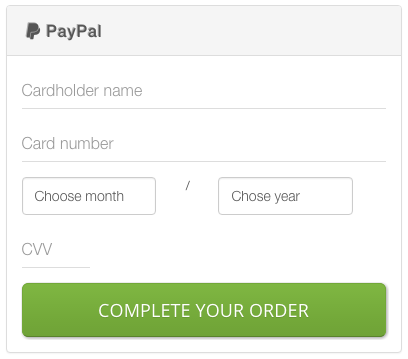
\includegraphics[width=0.6\textwidth]{figuras/payment/credit_card_form.png}
			\caption{Formulario de la tarjeta de crédito para realizar el pago utilizando \PPPaymentProNAME.}
			\label{figure:checkout:payment:paypal_payflow:form}
		\end{figure}

		%TODO: agregar referencia a la interfaz de orde de compra.
		Una vez finalizado este proceso, se creará una orden de compra, la cual podría ser consultado en la interfaz de ordenes.